\documentclass[11pt, oneside]{article}   	% use "amsart" instead of "article" for AMSLaTeX format
\usepackage{geometry}                		% See geometry.pdf to learn the layout options. There are lots.
\geometry{letterpaper}                   		% ... or a4paper or a5paper or ... 
%\geometry{landscape}                		% Activate for for rotated page geometry
%\usepackage[parfill]{parskip}    		% Activate to begin paragraphs with an empty line rather than an indent
\usepackage{graphicx}				% Use pdf, png, jpg, or eps� with pdflatex; use eps in DVI mode
								% TeX will automatically convert eps --> pdf in pdflatex		
\usepackage{amssymb}
\usepackage{amsmath}
\usepackage{parskip}
\usepackage{color}

\title{Stokes problems (math24.net)}
%\author{The Author}
%\section{}
% \subsection*{R code}
\date{}							% Activate to display a given date or no date

\graphicspath{{/Users/telliott_admin/Dropbox/Tex/png/}}

% \begin{center} 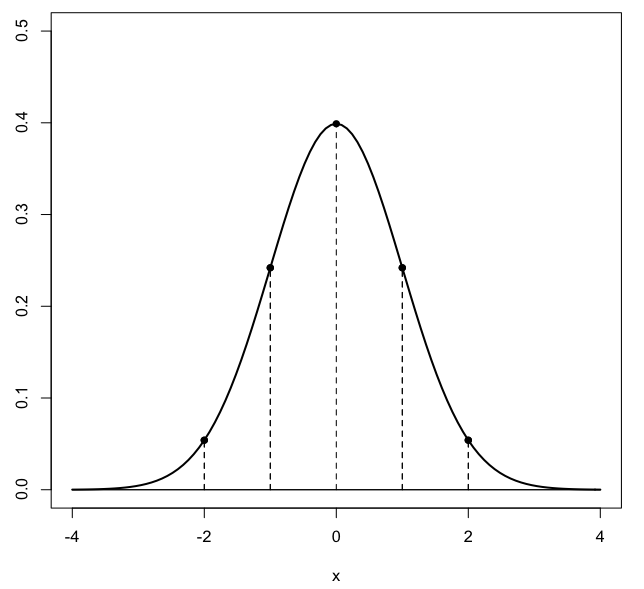
\includegraphics [scale=0.4] {gauss3.png} \end{center}
% \begin{bmatrix} a  &  b \\ c  &  d \end{bmatrix}
% \bigg |_

\begin{document}
\maketitle
\large
%\noindent

Stokes Theorem is:
\[ \oint_C \mathbf{F} \cdot \mathbf{r} = \iint_R (\nabla \times \mathbf{F}) \cdot \hat{\mathbf{n}} \ dS \]

\subsection*{Problem 1}

Given 
\[ \mathbf{F} = \langle yz,xz,xy \rangle \]
Show that the integral
\[ \oint_C yz \ dx + xz \ dy + xy \ dz = 0 \]
over \emph{any} closed curve $C$.

One way to do this is to guess the potential function for which $\mathbf{F} = \nabla f$.
\[ f(x,y,z) = xyz \]
fulfills this criterion.  Since this is true, the curl of $\mathbf{F}$ must be zero.  By Stokes theorem, the integral is zero for any closed curve $C$.

A second approach is to actually calculate the curl
\[ \nabla \times \mathbf{F} = \langle R_y - Q_z, P_z - R_x, Q_x - P_y \rangle \]
\[ = \langle x - x, y - y, z - z \rangle = \langle 0, 0, 0 \rangle \]
and the dot product with \emph{any} $\hat{\mathbf{n}}$ is zero.

\subsection*{Problem 2}
Evaluate
\[ \oint_C (y + 2z)dx + (x + 2z)dy + (x + 2y)dz \]
where $C$ is the intersection of the unit sphere $x^2 + y^2 + z^2 = 1$ with the plane $x + 2y + 2z = 0$.  This looks fairly hard at first.  How to parameterize this curve?  But we start by calculating
\[ \nabla \times \mathbf{F} = \langle 2 - 2, 2 - 1, 1 - 1 \rangle = \langle 0, 1, 0 \rangle  \]
What is $\hat{\mathbf{n}} \ dS$?  Our surface is a part of the plane.  Notice that $(0,0,0)$ is a solution of the equation for the plane, so it goes through the origin.  Therefore, the intersection is a circle of radius $1$.  The plane has normal vector $\mathbf{n} = \langle 1,2,2 \rangle$ and \emph{unit normal} $\hat{\mathbf{n}} = 1/3 \ \mathbf{n}$ so
\[ (\nabla \times \mathbf{F} ) \cdot \hat{\mathbf{n}} = \frac{2}{3} \]
Thus we have 
\[ \iint_R (\nabla \times \mathbf{F}) \cdot \hat{\mathbf{n}} \ dS =  \iint_R \ \frac{2}{3} \ dS \]
which is just two-thirds the area of the unit circle, or $4/3 \pi$.

\subsection*{Problem 3}

Evaluate 
\[ \oint_C y^3 \ dx - x^3 \ dy + z^3 \ dz \]
where $C$ is the intersection of the cylinder $x^2 + y^2 = a^2$ and the plane $x+ y + z = b$.

The normal vector to the plane is $\mathbf{n} = \langle 1,1,1 \rangle$.  We could certainly parametrize the curve in terms of the angle $\theta$ going around the cylinder.  $z$ would move from a minimum at $\theta = \pi/4$ to a maximum on the other side of the circle.

Let's try the curl first.
\[ \mathbf{F} = \langle y^3, -x^3 , z^3 \rangle \]
\[ \nabla \times \mathbf{F} = \langle R_y - Q_z, P_z - R_x, Q_x - P_y \rangle \]
\[ = \langle 0, 0, -3x^2 - 3y^2 \rangle \]

Using the equation of the surface $z = b - x - y$, we get that $f_x =  -1 = f_y$ so 

\[ \hat{\mathbf{n}} \ dS = \langle -f_x,-f_y,1 \rangle \ dx \ dy \] 

and
\[ (\nabla \times \mathbf{F} ) \cdot \hat{\mathbf{n}} \ dS = -3x^2 - 3y^2 \ dx \ dy \]

\[ \iint_R (\nabla \times \mathbf{F}) \cdot \hat{\mathbf{n}} \ dS =  \iint_R -3x^2 - 3y^2 \ dx \ dy \]
\[ = -3 \iint_R x^2 + y^2 \ dx \ dy \]
We need to integrate this over a circle of radius $a$,
so switch to polar coordinates
\[ = -3 \int \int r^2 \ r \ dr \ d \theta \]
\[ = -3 \  \int \frac{1}{4} a^4 \ d \theta \]
\[ = -\frac{3}{2} \pi a^4 \]









\end{document}  